
\begin{frame}[noframenumbering]
  \frametitle{Appendix I} 
%	bla bla bla bla bla bla bla bla \\ bla bla bla bla  bla bla bla bla 
%	\begin{right} 
	\centering
	\includegraphics[page=2, width=.6\textwidth]{../img/mindmap.pdf}
\end{frame}
%------------------------------------------------------
\begin{frame}[noframenumbering]
  	\frametitle{Appendix II}
%  
	Wir notieren:
%	
	\begin{align}
		r_1^2&= (x_1-x )^2 + (y_1-y )^2 + (z_1-z )^2\\
		r_2^2&= (x_2-x )^2 + (y_2-y )^2 + (z_2-z )^2\\
		r_3^2&= (x_3-x )^2 + (y_3-y )^2 + (z_3-z )^2\\
		\nonumber\\
		r_0^2&= (x_0-x )^2 + (y_0-y )^2 + (z_0-z )^2\\
		\nonumber\\
		r_{0k}^2&= (x_0-x_k )^2 + (y_0-y_k )^2 + (z_0-z_k )^2 \\
		\nonumber\\
		r(\Theta_k,n_k)&=\frac{\lambda}{2}\left(\Theta_k+n_k\right)
%		
	\end{align}
%
\end{frame}
%------------------------------------------------------
\begin{frame}[noframenumbering]
  	\frametitle{Appendix III}
%
Linearisierung des Modells.
%
\begin{align}
	r_{k}^2 &= (x-x_k)^2+(y-y_k)^2+(z-z_k)^2 \nonumber \\
	&=(x-x_k+x_0-x_0)^2+(y-y_k+y_0-y_0)^2+(z-z_k+z_0-z_0)^2 \nonumber \\
%	&=((x-x_0)-(x_k-x_0))^2+((y-y_0)-(y_k-y_0))^2+((z-z_0)-(z_k-z_0))^2 \nonumber \\ 
	%2 bin. Form
	&=(x-x_0)^2-2(x-x_0)(x_k-x_0)+(x_k-x_0)^2\underbrace{+\dots{}+\dots{}}_\text{y-\& z-Terme analog}
	\label{eq:tri_temp1}
%
\end{align}
%
Durch Umstellen erhalten wir:
\begin{align}
(x-x_0)(x_k-x_0)+\dots{}+\dots{}&=\phantom{-}\frac{1}{2}[(x_k-x_0)^2 +(x-x_0)^2 +\dots{}+\dots{}-r_k^2]\nonumber
%
\end{align}
%
\begin{multline}
	(x-x_0)(x_k-x_0)+(y-y_0)(y_k-y_0)+(z-z_0)(z_k-z_0)= \\\frac{1}{2}[\underbrace{(x_k-x_0)^2+(z_k-z_0)^2+(y_k-y_0)^2}_\text{\boldmath{$d_{kj}^2$}}
	\\+\underbrace{(x-x_0)^2+(y-y_0)^2 +(z-z_0)^2}_\text{\boldmath{$r_j^2$}}-r_k^2]
\end{multline}
	
%
\end{frame}
%------------------------------------------------------
\begin{frame}[noframenumbering]
  	\frametitle{Appendix IV}
%
\begin{align*}
a_{0k} :&= \frac{1}{2}d_{kj}^2\\
a_1 :&= \frac{\lambda^2}{8}\\
a_2 :&= a_1\frac{1}{\pi}\\
a_{3kj} :&= a_1\frac{1}{(2\pi)^2}(\Theta_j^2-\Theta_k^2)
\end{align*}
\end{frame}
%------------------------------------------------------
\begin{frame}[noframenumbering]
  	\frametitle{Appendix V}
%
  \begin{center}
  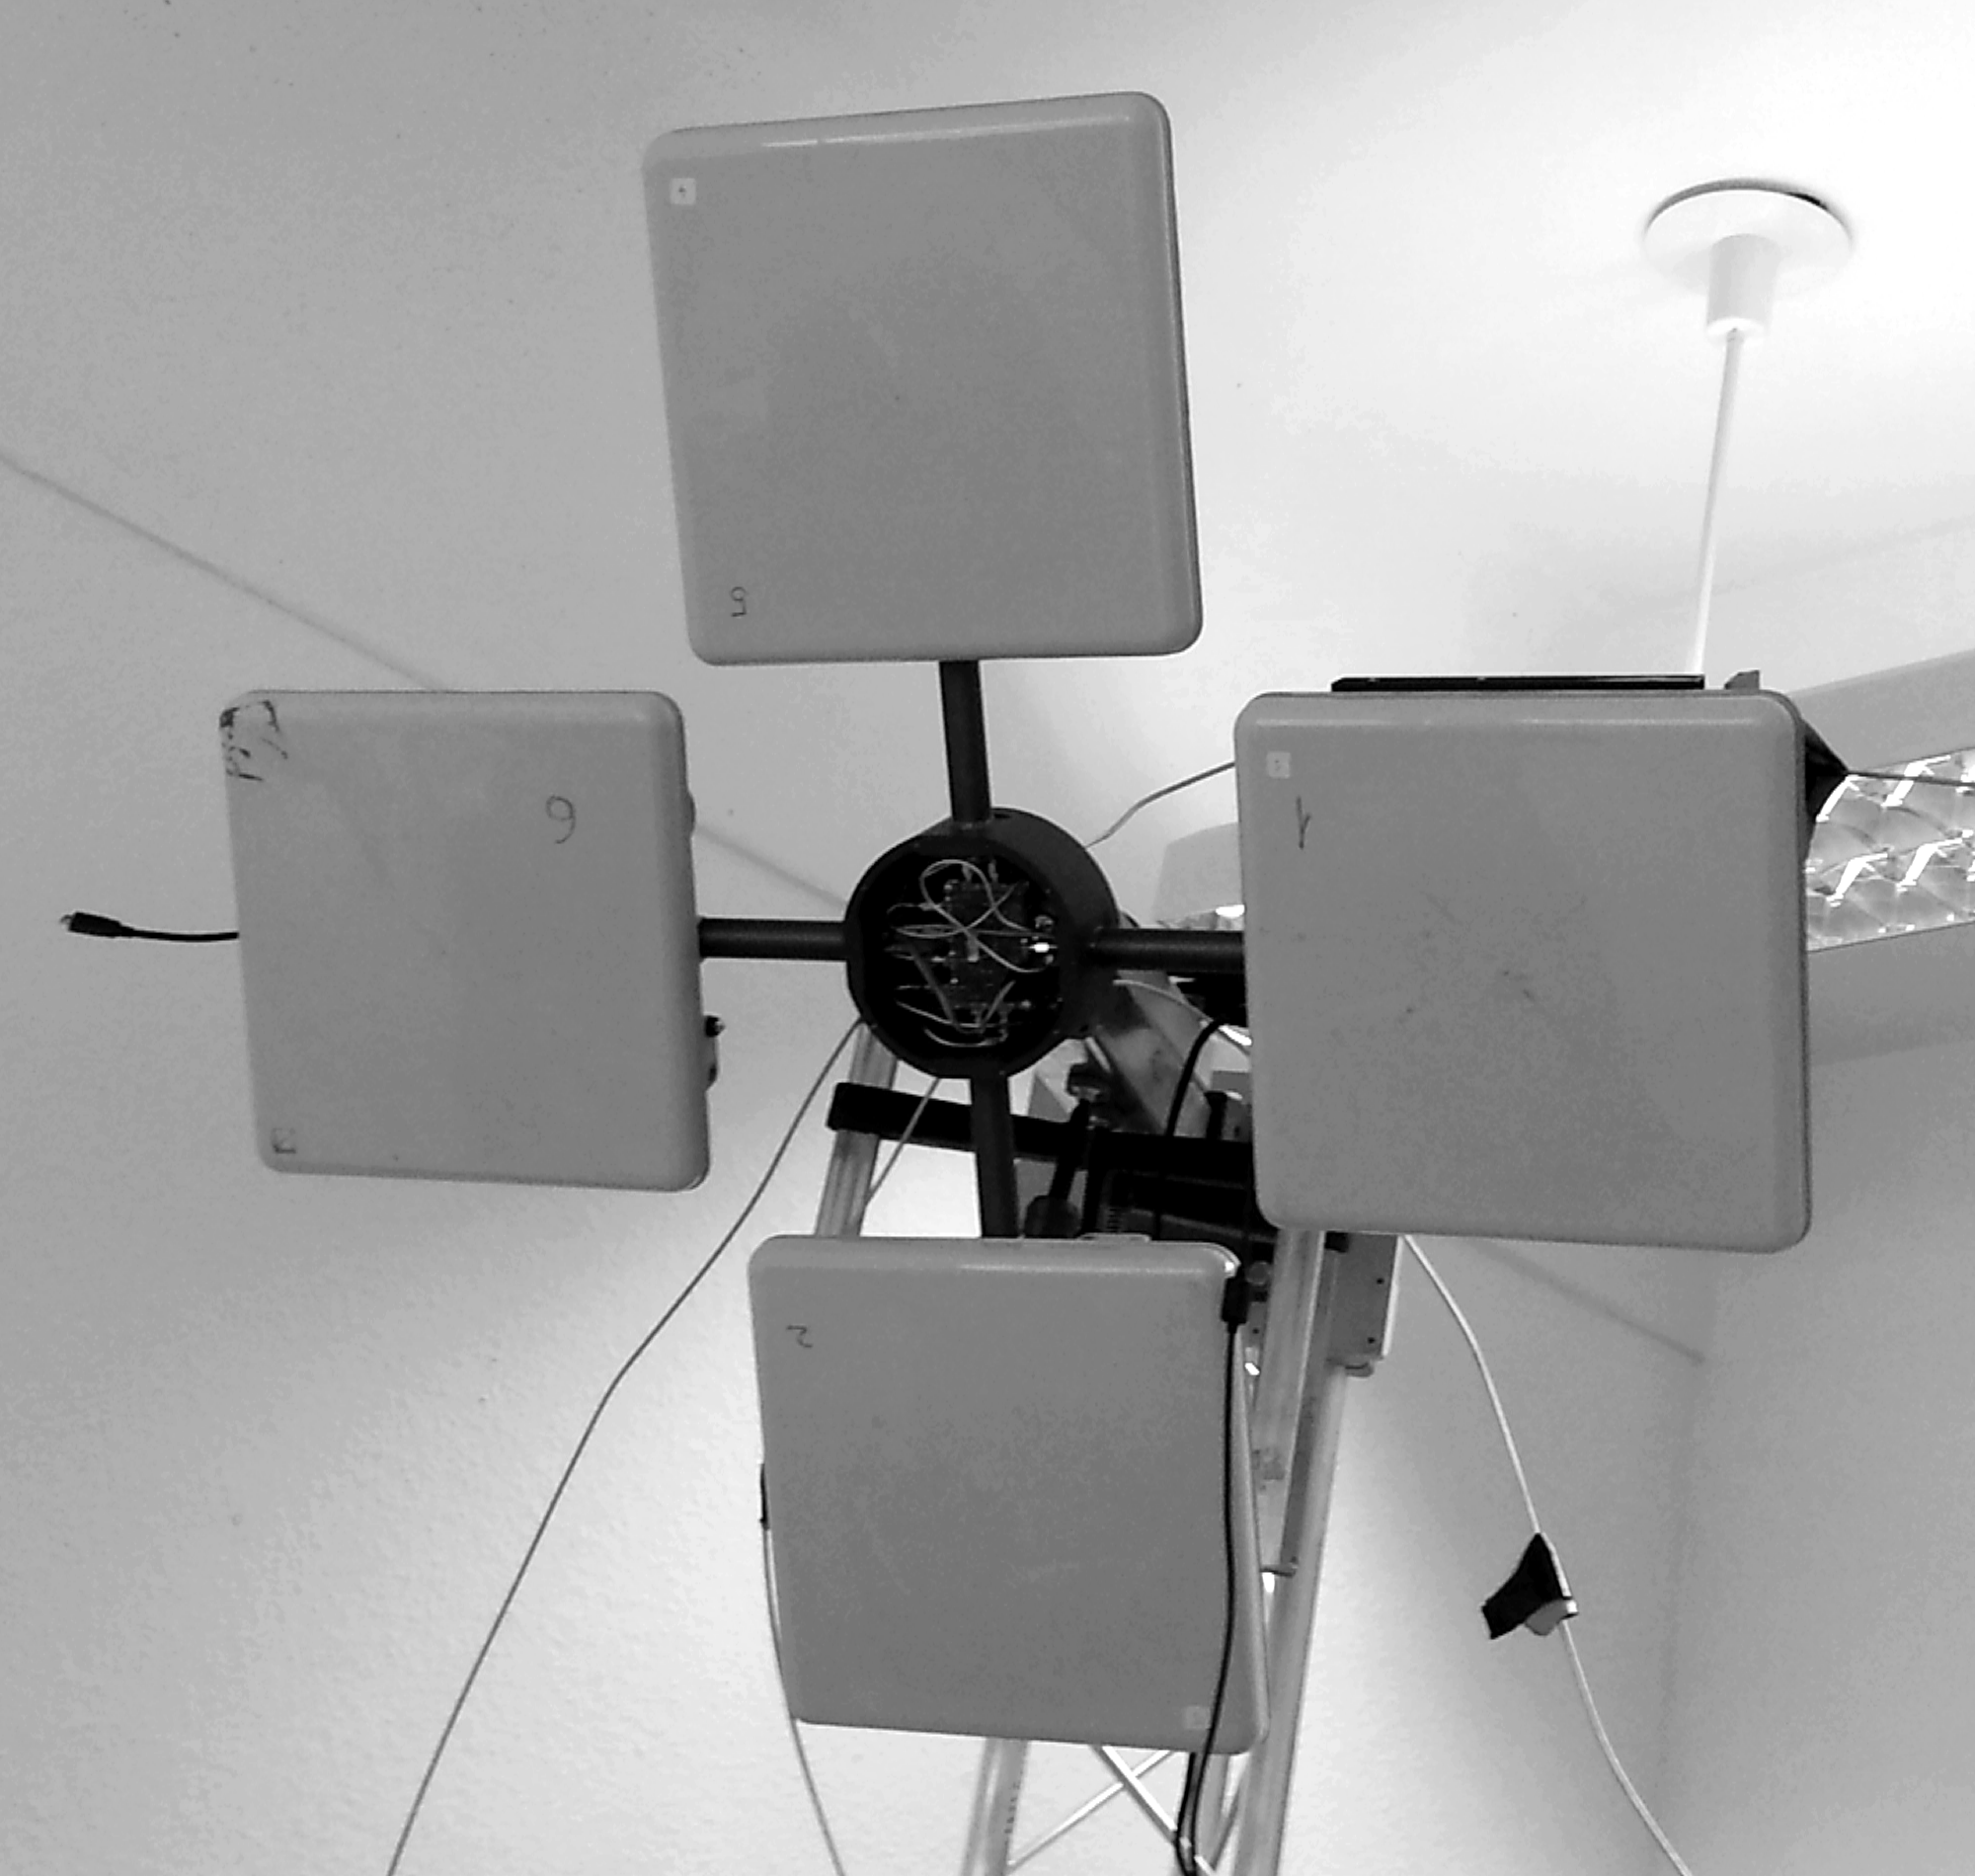
\includegraphics[width=.3\textwidth]{../img/4AntennaSetup_small.png}
  \qquad
  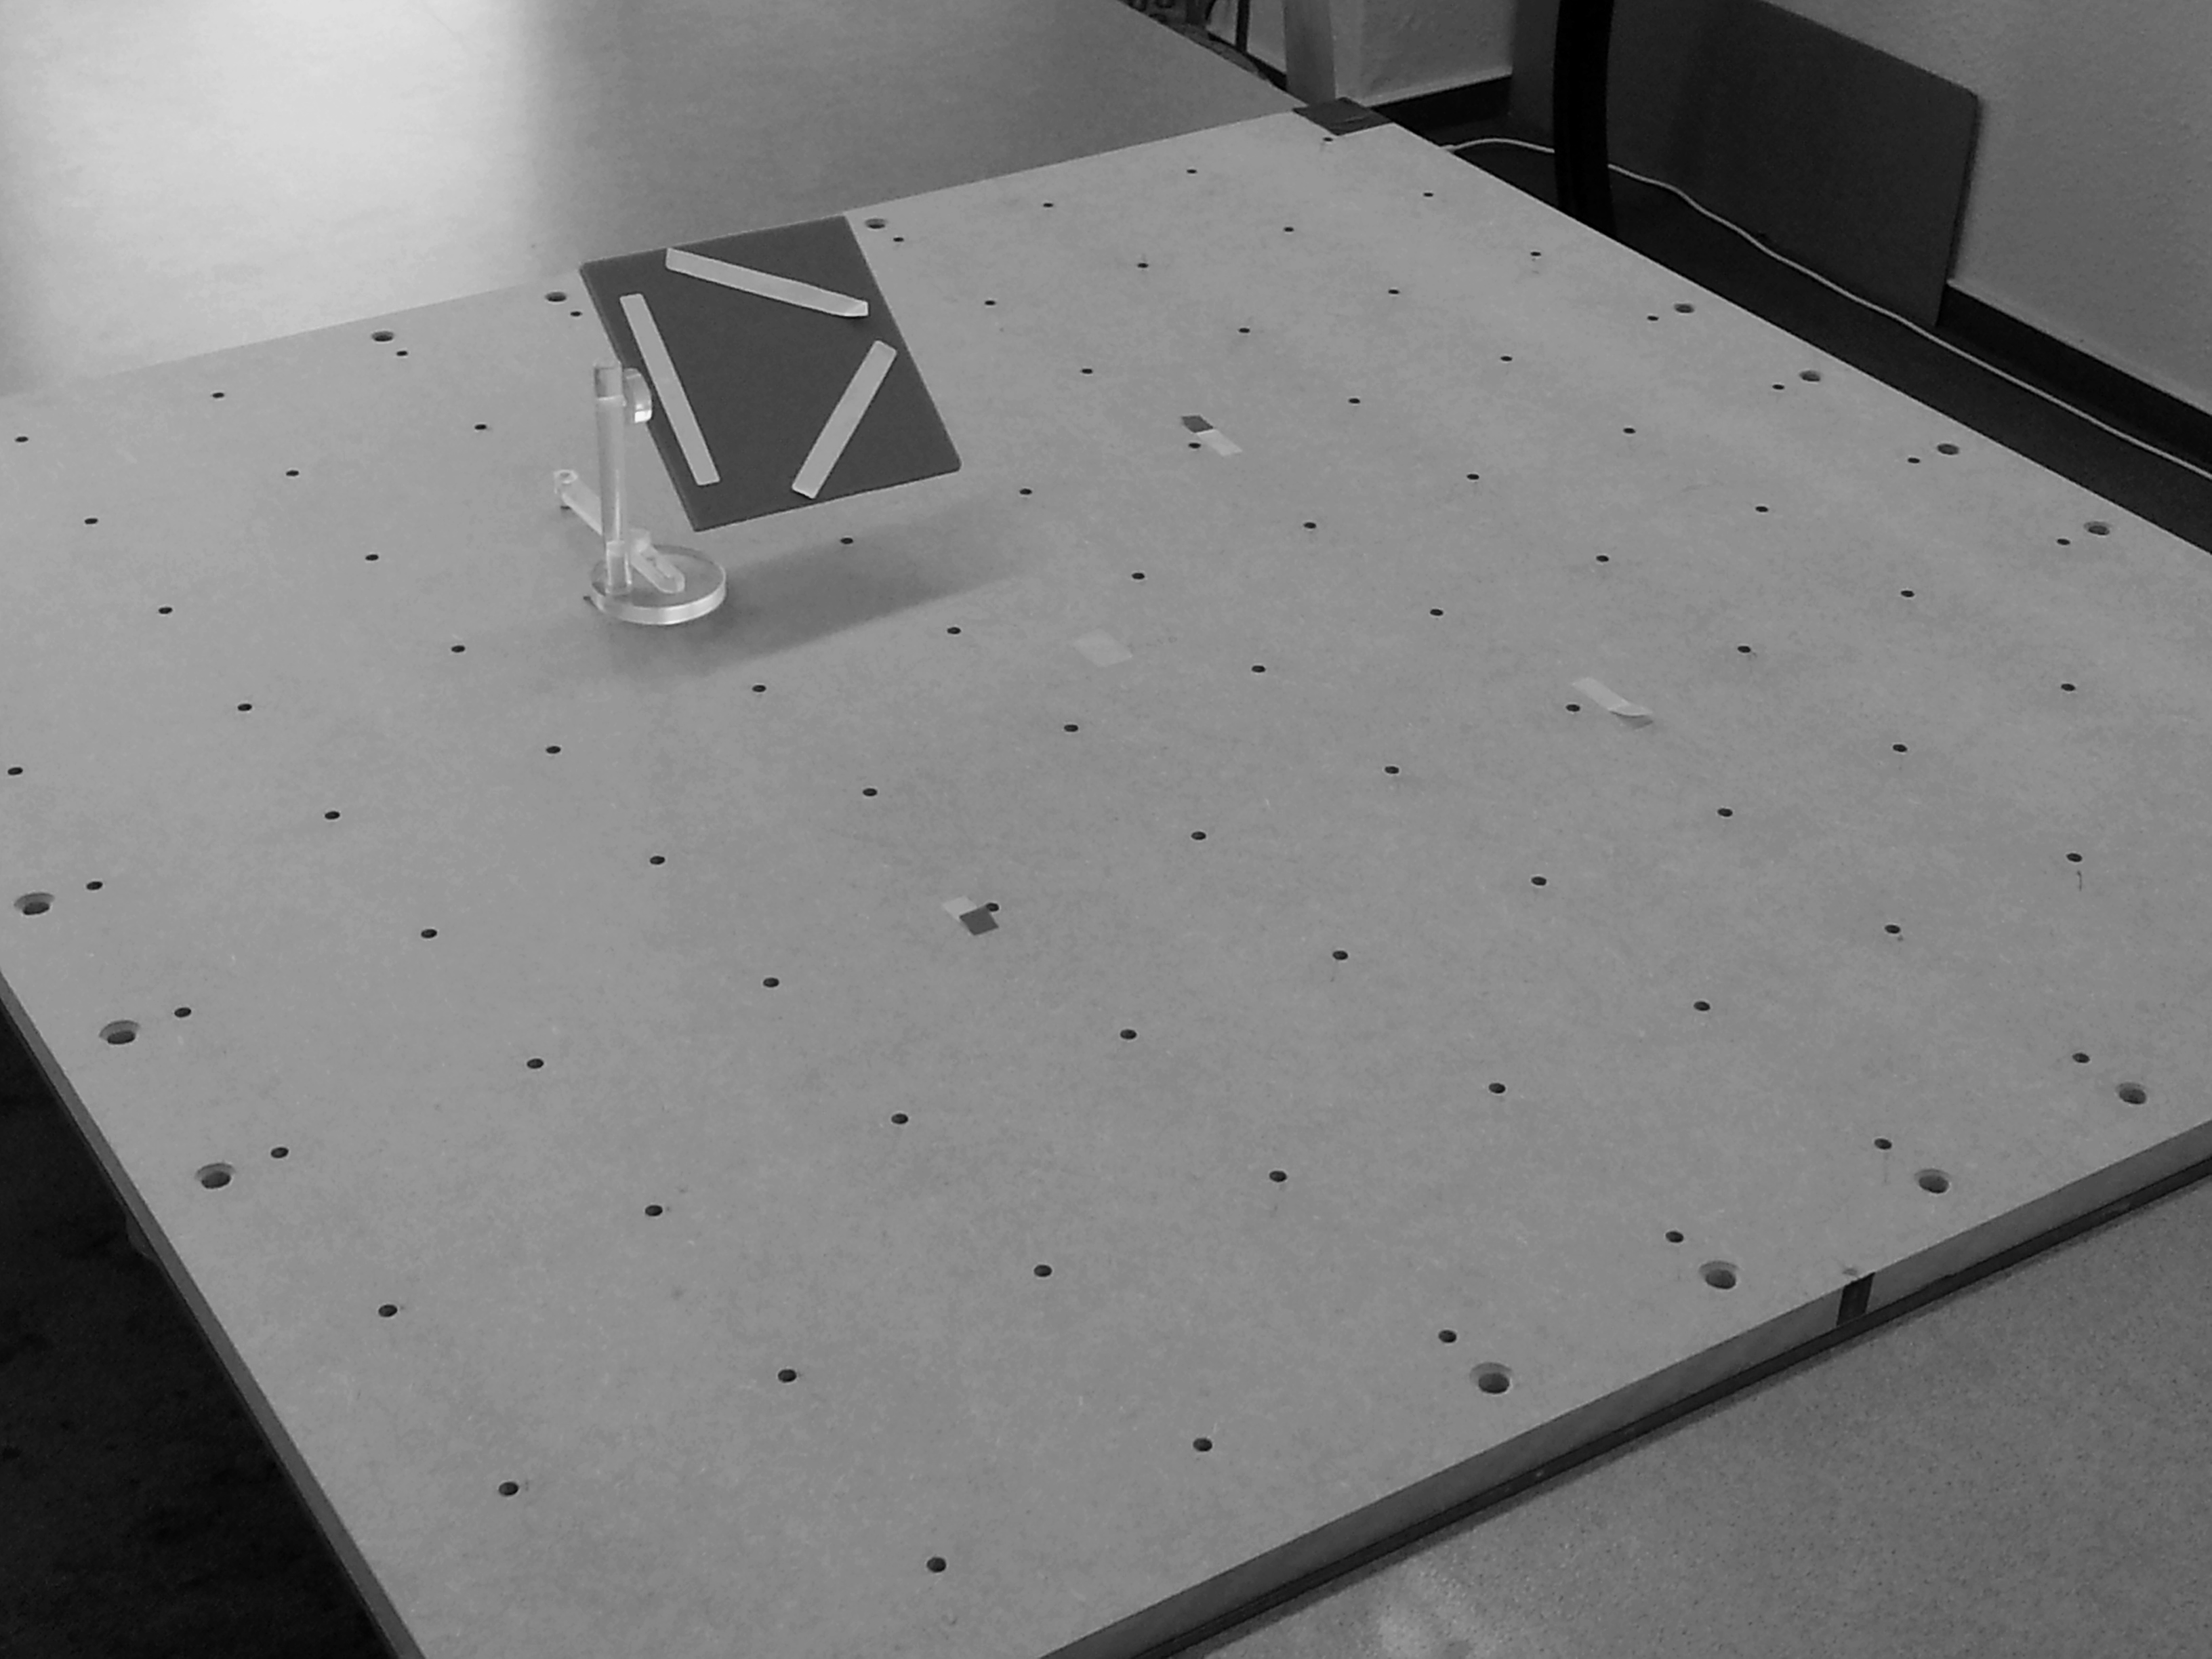
\includegraphics[width=.3\textwidth]{../img/Calibration_Plate1.png}
%  \qquad
%  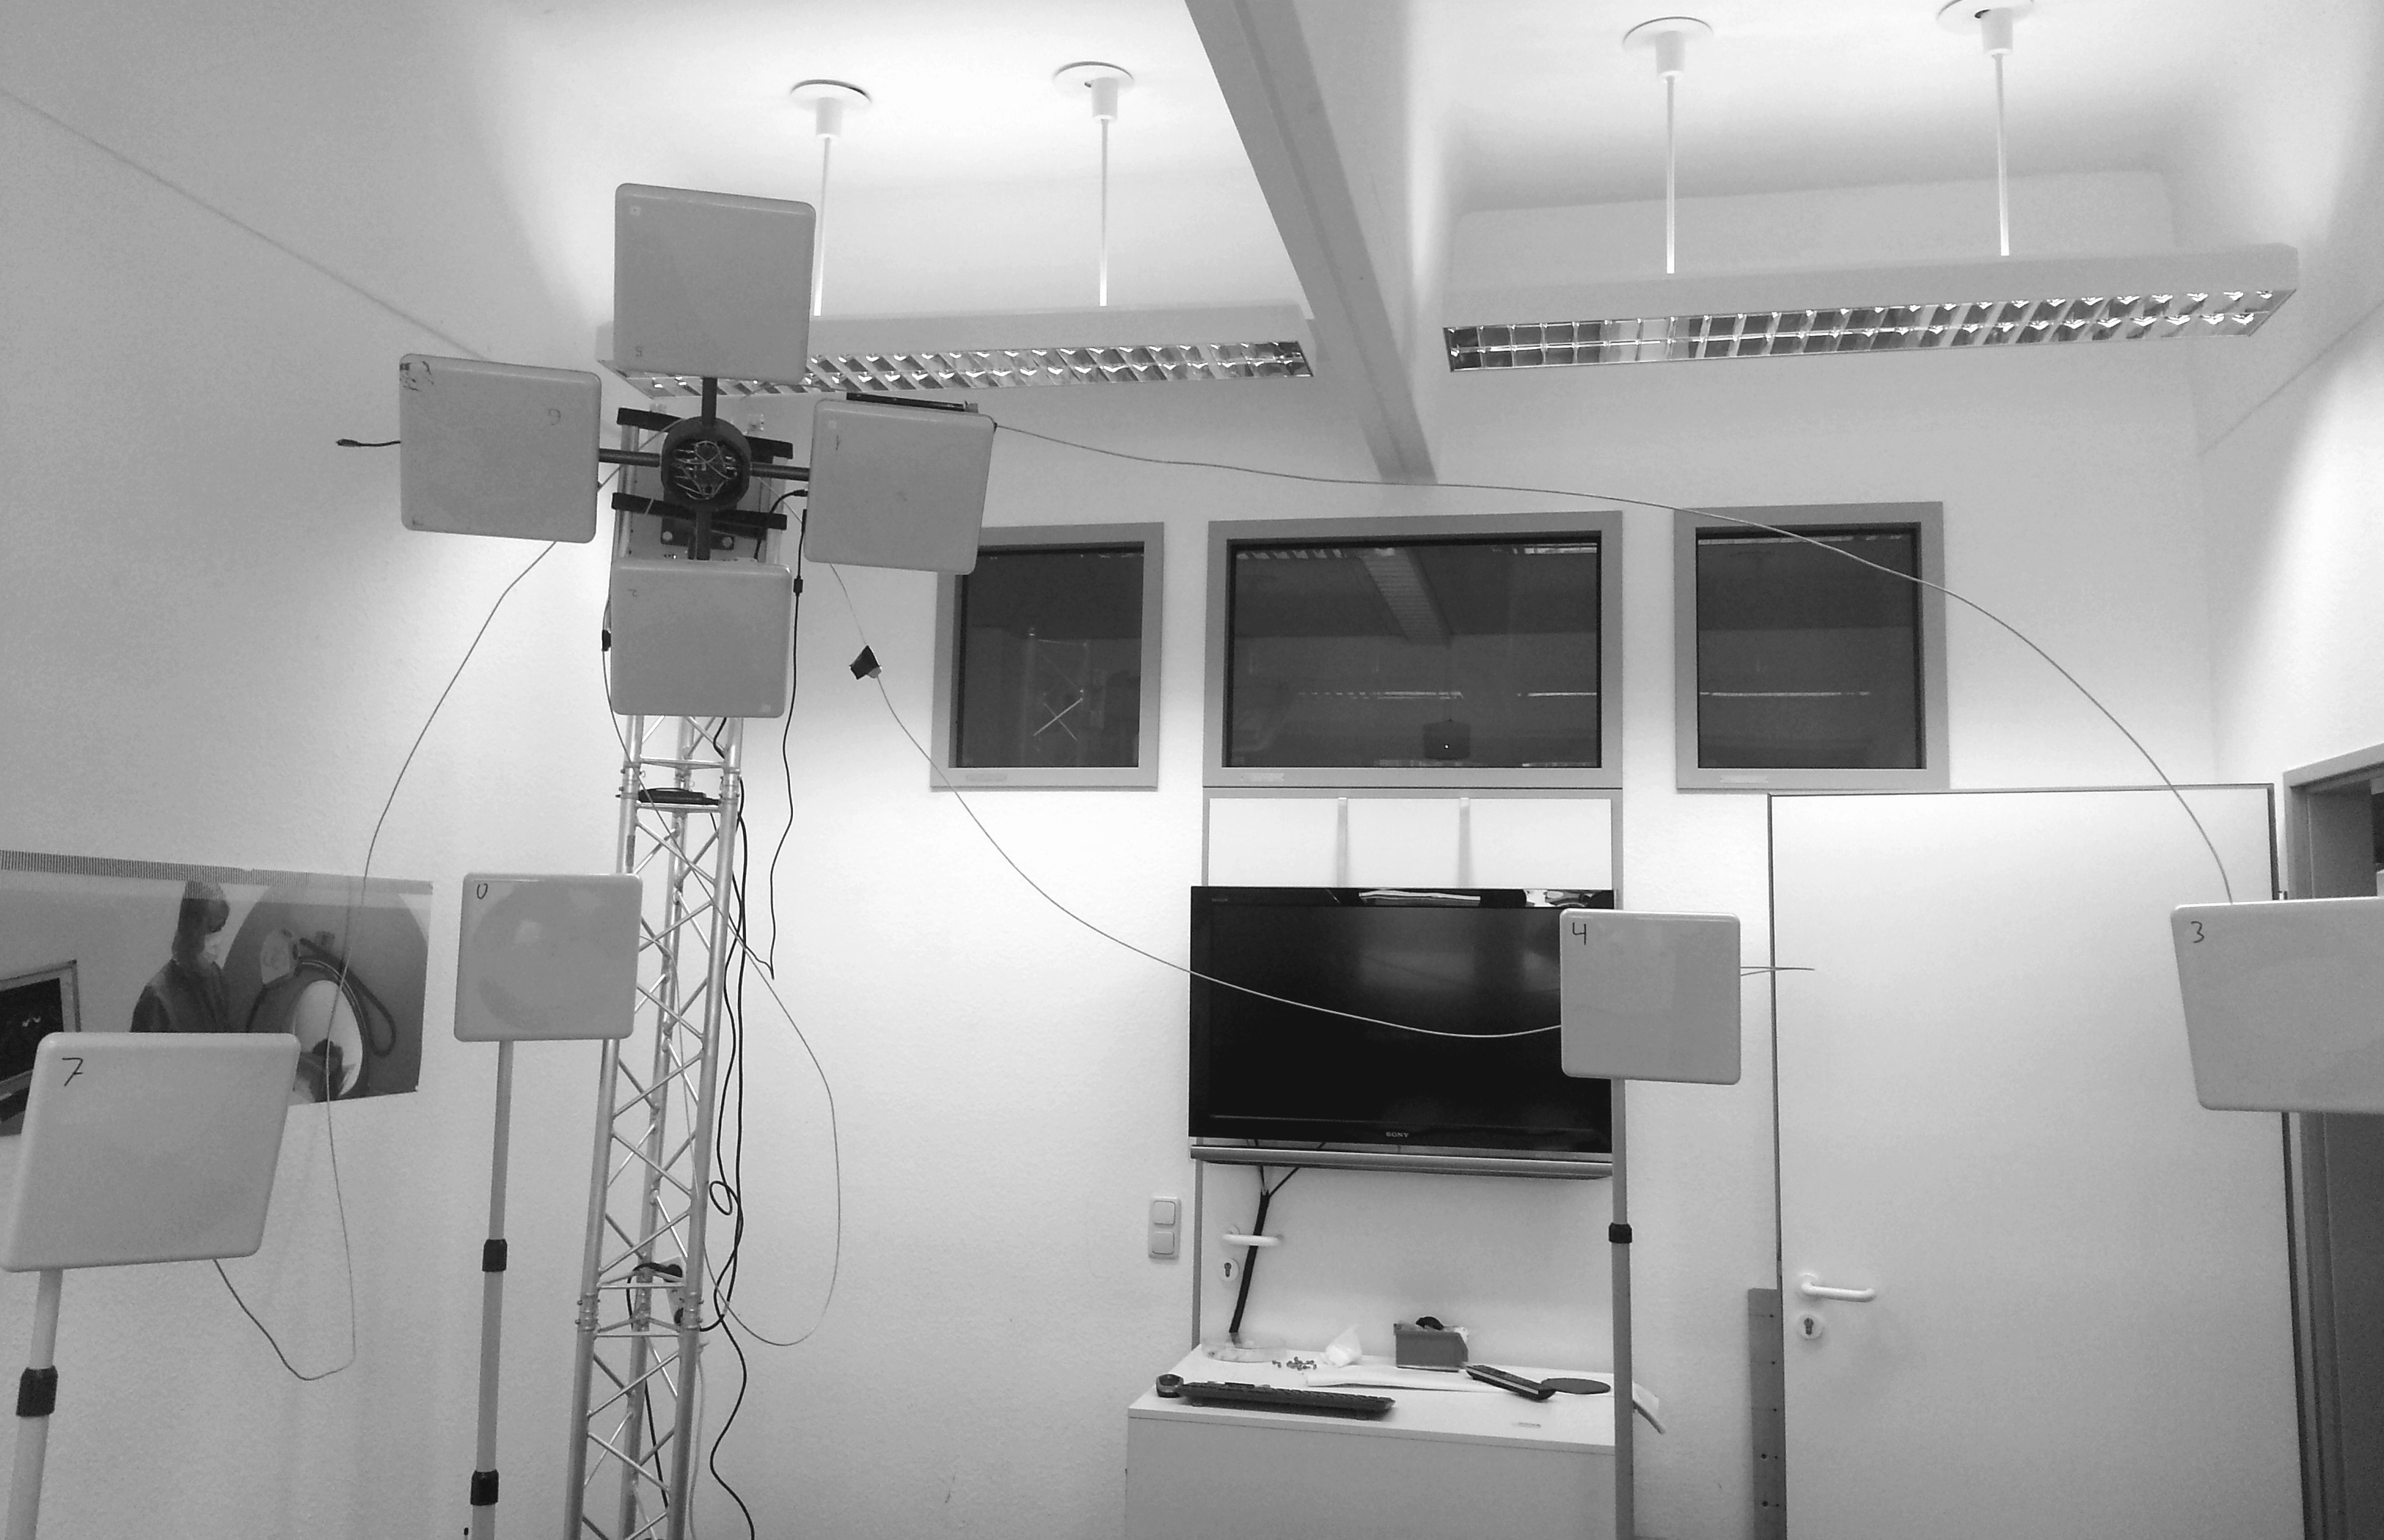
\includegraphics[width=.3\textwidth]{../img/RFID-Okto.png}
  \end{center}
\end{frame}
%------------------------------------------------------
%\begin{frame}
%  	\frametitle{Modellierung 2}
%%  
%	Wir notieren:
%%	
%	\begin{align}
%		r_1^2&= (x_1-x_{Tag} )^2 + (y_1-y_{Tag} )^2 + (z_1-z_{Tag} )^2\\
%		r_2^2&= (x_2-x_{Tag} )^2 + (y_2-y_{Tag} )^2 + (z_2-z_{Tag} )^2\\
%		r_3^2&= (x_3-x_{Tag} )^2 + (y_3-y_{Tag} )^2 + (z_3-z_{Tag} )^2\\
%		\nonumber\\
%		r_0^2&= (x_0-x_{Tag} )^2 + (y_0-y_{Tag} )^2 + (z_0-z_{Tag} )^2\\
%		\nonumber\\
%		r_{0k}^2&= (x_0-x_k )^2 + (y_0-y_k )^2 + (z_0-z_k )^2 \\
%		\nonumber\\
%		r(\Theta,n)&=\frac{\lambda}{2}\left(\Theta+n\right)
%%		
%	\end{align}
%%
%\end{frame}
%------------------------------------------------------
%\begin{frame}
%  	\frametitle{Modellierung 3}
%%--
%	Gleichung der Form:
%	\[\mathbf{A}\mathbf{x}=\mathbf{b}\]  
%%--
%	,wobei:
%	\begin{multline}
%	\mathbf{A}=\\
%	\left(
%		\begin{array}{cccccccccc}
%			x_1-x_0 & y_1-y_0 & z_1-z_0 & -a_1 & 0 & 0 & -a_2\Theta_0 & a_2\Theta_1 & 0 & 0 \\
%			x_2-x_0 & y_2-y_0 & z_2-z_0 & 0 & -a_1 & 0 & -a_2\Theta_0& 0 & a_2\Theta_2 & 0 \\
%			x_3-x_0 & y_3-y_0 & z_3-z_0 & 0 & 0 & -a_1 & -a_2\Theta_0& 0 & 0 & a_2\Theta_3
%		\end{array}
%	\right) \nonumber
%	\end{multline}
%%--
%	und
%	\begin{multline}
%	\mathbf{x}=\\
%	\left(
%		\begin{array}{cccccccccc}
%			x-x_0 & y-y_0 & z-z_0 &	n_0^2-n_1^2	& (\dots)	&	n_0^2-n_3^2 & n_0 & n_1	& (\dots) &	n_3	
%		\end{array}
%	\right)^T\nonumber
%	\end{multline}
%%--
%	\begin{multline}
%		\mathbf{b}=\\
%		\left(
%			\begin{array}{c}
%				a_{0k}-a_{3kj} 
%			\end{array}
%			\right)^T
%			= c_{kj}'\nonumber
%		\end{multline}
%%--		
%\end{frame}